\documentclass[border=10pt]{standalone}
\usepackage{tikz}
\usetikzlibrary{arrows.meta, shapes, calc}

\begin{document}
\begin{tikzpicture}[scale=1.5, >=Stealth]

% Define grid and axes
\draw[step=0.1, gray!50, very thin] (0,0) grid (2,2);
\draw[thick, blue!80!black] (0,0) -- (2,0) -- (2,2) -- (0,2) -- cycle;

% Axes
\draw[thick, ->] (0,0) -- (2.2,0) node[below right] {$u$};
\draw[thick, ->] (0,0) -- (0,2.2) node[above left] {$v$};

% Label origin
\node[below left, green!50!black] at (0,0) {$Q$};

% Mark points on axes
\draw[thick, blue!80!black] (2/3,0) -- (2/3,0.05) node[below] {$\frac{2}{3}$};
\draw[thick, blue!80!black] (0,2/3) -- (0.05,2/3) node[left] {$\frac{2}{3}$};
\draw[thick, blue!80!black] (2,0) -- (2,0.05) node[below] {$2$};
\draw[thick, blue!80!black] (0,2) -- (0.05,2) node[left] {$2$};

% Draw blue squares
\fill[blue!30] (0,0) rectangle (2/3,2/3);
\fill[blue!30] (2/3,2/3) rectangle (2/3 + 2/9, 2/3 + 2/9);
\fill[blue!30] (2/3 + 2/9, 2/3 + 2/9) rectangle (2/3 + 2/9 + 2/27, 2/3 + 2/9 + 2/27);
\fill[blue!30] (2/3 + 2/9 + 2/27, 2/3 + 2/9 + 2/27) rectangle (2/3 + 2/9 + 2/27 + 2/81, 2/3 + 2/9 + 2/27 + 2/81);

% Fill the rest with pink
\fill[pink!80] (0,0) rectangle (2,2);
\fill[white] (0,0) rectangle (2/3,2/3); % remove the first blue square
\fill[white] (2/3,2/3) rectangle (2/3 + 2/9, 2/3 + 2/9); % remove second
\fill[white] (2/3 + 2/9, 2/3 + 2/9) rectangle (2/3 + 2/9 + 2/27, 2/3 + 2/9 + 2/27); % remove third
\fill[white] (2/3 + 2/9 + 2/27, 2/3 + 2/9 + 2/27) rectangle (2/3 + 2/9 + 2/27 + 2/81, 2/3 + 2/9 + 2/27 + 2/81); % remove fourth

% Add the label
\node[draw, thick, rounded corners, fill=white, text=black, align=left, font=\small] at (1.5,0.5) {
  $S = \dfrac{2}{3} + \dfrac{2}{9} + \dfrac{2}{27} + \cdots$
};

\end{tikzpicture}
\end{document}